% Copyright 2011 Nadia Davidson 
% for The ARC Centre of Excellence in Coherent X-ray Science. 

\documentclass[]{cxs-software}
\usepackage{graphicx}
\usepackage{hyperref}
\usepackage{eurosym}
\usepackage{pifont}
%\usepackage{tocloft}
\usepackage{amsmath}
\usepackage{subfigure}
\usepackage{fancyhdr}
\usepackage{fancyvrb}
\usepackage{booktabs}
\usepackage{comment}
\usepackage{import}
\usepackage{listings}
\usepackage{tikz}
\usepackage{html}


%\usepackage{dirtree}
%\renewcommand*\DTstylecomment{\textsf}

%\begin{htmlonly}
%  \usepackage{verbatim}
%  \providecommand{\lstlisting}[2][]{\verbatim{#2}}
%  \renewcommand*{\lstlisting}{\verbatim}
%\end{htmlonly}
\lstnewenvironment{myverbatim}{}{}

\RequirePackage[dvips]{color}

\definecolor{mycolour}{rgb}{0.05,0.2,0.5}
\definecolor{gray}{rgb}{0.9,0.9,0.9}
\definecolor{darkgray}{rgb}{0.3,0.3,0.3}

%\usepackage{doxygen}
\pagestyle{fancy}

\lstset{
language=C++,
breakatwhitespace=true,
basicstyle=\ttfamily\color{mycolour},     % Code font, Examples: \footnotesize, \ttfamily
commentstyle=\color{darkgray},            % Comments font
backgroundcolor=\color{gray},
basewidth=0.5em,
breaklines=true,
}   

\usetikzlibrary{shapes.arrows,chains,positioning}
\def\pgfsysdriver{pgfsys-tex4ht.def}

%\usepackage{color,fancyvrb}
%\renewcommand\FancyVerbFormatLine[1]
%{\colorbox{gray}{\makebox[\linewidth][l]{#1}}}

%\DefineShortVerb{\!}

%\makeatletter
%\renewcommand*\l@section{\bf{\color{mycolour}\sffamily{#1}}}
%\renewcommand*\l@subsection{\bf{\color{mycolour}\sffamily{#1}}}
%\renewcommand*\l@subsubsection{\bf{\color{mycolour}\sffamily{#1}}}
%\makeatother

%\makeatletter
%\newcommand{\mysection}[1]{%
%  \section*{\bf{\color{mycolour}\sffamily{#1}}}}
%\newcommand{\mysubsection}[1]{%
%  \subsection*{\bf{\color{mycolour}\sffamily{#1}}}}
%\newcommand{\mysubsubsection}[1]{%
%  \subsubsection*{\color{mycolour}\sffamily{#1}}}
%\makeatother

\begin{document}
\sffamily

\vspace{6cm}

\maketitle

\setcounter{tocdepth}{3}
%\tableofcontents\pdfbookmark[0]{Table of Contents}{toc}
\tableofcontents

\newpage


%\section{Introduction}

%The high resolution imaging of finite nano-scale objects has been
%shown to be possible due to .........
%the developement of Coherent Diffractive
%Imaging (CDI) techniques~\cite{}.

%Wavelength limited resolution...

%lense-less X-ray imaging techniques have proved to
%be a promising technique for imaging nano-scale biological objects.

%The phase information is recovered computationally, through use of
%iterative algorithms~\cite{}. 

%The rapid developement in theory and experimentation in this field has
%created a need for common software tools within the CDI community.
%HAWKE~\cite{}, a plane-wave CDI reconstruction package, was was
%developed for this purpose. The need for Fresnel coherent diffractive
%imag



%In this paper we describe a computer program 

%.which provide a user
%friendly, reliable and fast method for reconstructing X-ray
%diffraction data.


%The program extends upon this existing software, by providing:
%\begin{itemize}
%\item A full choice of iterative algorithms, including customised
%  algorithms. In~\cite{} it was demonstrated that all reconstruction
%  algorithms could be expressed through X combinations of projection
%  operators. ......
%\item Fresnel Coherent Diffractive Imaging algorithms~\cite{} have
%  been implemented.
%\item Ptychographic~\cite{} and Phase-Diverse~\cite{} CDI have also
%  been implemented.
%\end{itemize}


%The software consists of a C++ library, interface to IDL, command-line
%tools in addition to example code and documentation. 

%......

%- motivation
%- review of similar software
%- goals and users


\section{Overview}

In the development of experimental infrastructure, software is an
important element which is often overlooked. For X-ray Coherent
Diffractive Imaging (CDI), in particular, computational inversion of
the measured diffraction intensity is an integral part of the image
reconstruction process. The proliferation of phase retrieval
algorithms has created the need for common software tools which
encompass all these approaches. The DIXE (Diffractive Imaging for
X-rays and Electrons) software package aims to provide a set of phase
retrieval tools which are robust, efficient and available to the wider
CDI community.

In this documentation, we introduce the software package, DIXE (also
known as cxs-software), which is able to reconstruct and simulate
X-ray diffraction data for plane-wave, Fresnel, ptychographic and
phase-diverse CDI. To the best of our knowledge, this is the first
standard software package which includes all of these different
approaches. The software allows for any choice of iterative algorithm,
including customized algorithms, and also includes the 'shrinkwrap'
algorithm. For Fresnel CDI, additional complex constraints on the
transmission function may also be used. The software consists of a C++
library, binding to IDL and command-line tools, in addition to example
code and documentation. It has been tested on the Mac, Windows and
Ubuntu operating systems. It is issued under the GNU public license.

It is assumed that readers of this manual are familiar with the
relevant literature describing the CDI algorithms implemented in \name
and we will therefore not repeat this information here. Please refer
to any of the reviews~\cite{} for more information on CDI. We intend
that this manual is used in the following ways:
\begin{itemize}
\item New users should follow the instructions provided for
  installation, Section \ref{installation}, followed by ``Getting
  Started'', Section \ref{getting started}.
\item The remainder of the manual is provided as a reference for users
  who are already familiar with the code. Section \ref{how to}, ``How
  to'', gives instructions on how to complete specific tasks and
  control the CDI reconstruction. The appendices document the
  important routines, functions and classes provided by the \name
  library.
\end{itemize}
This version of the software is a developement (beta) version and we
welcome feedback on any aspect of the software package: functionality,
installation, documentation etc. Please email
cxs-software@physics.unimelb.edu.au for questions or comments.

%%%%%%%%%%%%%%%%%%%%%%%%%%%%%%%%%%%%%%%%%%%%%%%%%%%%%%%%%%%%%%%%%%%%%%%%%%%%

\newpage
\section{Installation Instructions}
\label{installation}

The software is available for download from the software website as either,
\begin{itemize}
\item a tar ball containing the software source code or
\item a pre-compiled Windows 32 bit binary file.
\end{itemize}

For Windows users who only wish to use the IDL capabilities or
command-line tools we recommend downloading the Windows binary file. For
all other users, we recommend downloading the source code package.

\subsection{Installing from Source Code}

\subsubsection{Linux}

Currently the code depends on several other libraries which will need to
be installed prior to installing this package:
\begin{itemize}
\item g++\cite{} - for compilation of C++ source code (we have tested against version 4.4.3)
\item fftw\cite{} - for fast Fourier transforms.
\item libtiff\cite{} - for reading and writing to tiff files.
\item HDF libraries\cite{} - for reading (and not yet writing to) hdf4
  files. Note that the hdf library depends on a few other libraries,
  which must also be installed.
\end{itemize}

Ubuntu users can easily install the external packages using the
synaptic package manager~\cite{}. The packages are named libfftw3-dev,
libtiff4-dev and libhdf4-dev.

Next, download our source code from the website and put it into an
appropriate directory. Unzip and untar the source code:
\begin{myverbatim}
  gunzip CXS.rel_0.4.tar.gz 
  tar -xvvf CXS.rel_0.4.tar
\end{myverbatim}

Change into the directory cxs\_software and compile the source code: 
\begin{myverbatim}
  cd cxs_software 
  ./configure 
  make
\end{myverbatim}

If ./configure doesn't finish by making a set of "Makefiles", the
dependent libraries probably haven't been installed correctly or
./configure does not know their location.

The result of compilation (if successful) are libraries and header
files (in the /lib and /include directories) and some example programs
which are ready to execute.

The source files in the examples/ directory e.g. PlanarCDI\_example.c
demonstrate how the libraries can be used within a user's own
code. The Makefile in examples/ shows how a user's code can be
compiled and the \name libraries linked.

\subsubsection{Mac}

\begin{enumerate}
\item Install Xcode\cite{}. This is a big download and you first have
  to register as a developer. Once installed, this is a nice text
  editor too.
\item Install fink\cite{} but following their instructions exactly.
  You can use fink like {\tt apt get} on linux to install the fftw and
  hdf packages. Make sure you select the correct releases of these.
\item Get and build the fftw, libtiff and hdf packages using fink
\item Download the \name source code from the website
\item Follow the install instruction for linux, except, replace ./configure with 
\begin{myverbatim}
  ./configure --with-fftw_inc=/sw/include --with-fftw_lib=/sw/lib CXX=''g++ -arch i386'' --with-mfhdf_inc=/sw/include --enable-checking
\end{myverbatim}
The ``--with'' flags will tell the compiler where to look for the
external packages.  The CXX="g++ -arch i386" relates to your
computer's architecture. This is for a late 2010 macbook pro running
10.6, try this, if it doesn't work, try looking up the relevant
information for your computer. %--enable-checking is just in case.
\item Type make, as in the linux instructions.
\end{enumerate}

\subsubsection{Windows with Cygwin}

Cygwin\cite{} provides a linux/unix type environment for Windows (the
interface is basically a unix style terminal). Installing the CXS
source code in this environment is very similar to installing it in
linux/unix and (in my opinion) makes modifying and recompiling the
code a bit easier than it would be in Windows otherwise. First you
will need to install cygwin. You can do this by going to
http://www.cygwin.com/, scrolling to the bottom of the page and
clicking on "Install or update now\ (using setup.exe)". Open setup.exe
and follow the installation instructions. Apart from the "Package
Selection" screen, used the default options. When you get to the
"Package Selection" screen leave "All" on "Default" and add the
additional packages by searching for them and then clicking on them:
\begin{itemize}
\item libhdf5-devel - These are libraries for reading hdf files.
\item gcc4-g++ - This is the c/c++ compiler I like to use.
\item make - This is used to automatically compile the package.
\item xemacs or emacs - This is a text/code editor
\item libfftw3-devel - This is a fast Fourier transform library.
\item libtiff-devel - This is a library for reading/writing tiff image files.
\item sunrpc
\item libjpeg-devel
\item zlib-devel
\end{itemize}

Note that you can update the packages which are installed after you've
installed cygwin just by clicking on setup.exe again (it remembers
which are installed). If you get an error during the post-installation
phase (error code 128) it maybe due to a virus checker interfering
with the cygwin installation.

Install the HDF4 libraries. There is no package for this in the
package manager so go to http://www.hdfgroup.org/release4/obtain.html
and download their cygwin binary. Unzip the file using the standard
windows tool and extract it into your home cygwin directory (which
should be something like
C:\textbackslash{}cygwin\textbackslash{}home\textbackslash{}your\_user\_name). The directory
hdf4.2.5-cygwin-szip should be made. The HDF library also needs the
szip library to work correctly. Download this from \\
http://www.hdfgroup.org/ftp/lib-external/szip/2.0/bin/cygwin/szip\_cygwin\_encoder.zip  \\
and also extract it into your home directory on cygwin.

Next, download the cxs software here and put it into your home
directory on cygwin \\
(C:\textbackslash{}cygwin\textbackslash{}home\textbackslash{}your\_user\_name). Open cygwin and
unzip and untar the package:
\begin{myverbatim}
$ gunzip CXS.rel_0.4.tar.gz 
$ tar -xvvf CXS.rel_0.4.tar 
\end{myverbatim}

When you type ``ls'' you should see the directory "cxs\_software" plus a
few others. Change into the cxs\_software directory:
\begin{myverbatim}
$ cd cxs_software 
\end{myverbatim}
Tell the package where your hdf and szip libraries files are located
(replace the "user\_name" with your cygwin user name):
\begin{myverbatim}
$ ./configure --with-mfhdf_lib=/home/"user_name"/hdf4.2.5-cygwin-szip/lib --with-mfhdf_inc=/home/"user_name"/hdf4.2.5-cygwin-szip/include --with-sz_lib=/home/"user_name"/szip_cygwin_encoder/lib 
\end{myverbatim}

If you get an errror, check that the paths given to configure are
correct; the lib directories should have files starting with "lib" and
the include directory should have files ending in ".h". If configure
worked correctly, compile the libraries and examples:
\begin{myverbatim}
$ make
\end{myverbatim}

Hopefully you won't get any errors and when you look in the lib/ and
include/ directories you will see some files. The libraries can be
useful if you ever need to create your own code (similar to the
examples). The examples show how the libraries can be used. 

\begin{comment}
--------------------------------------
Change into the example directory:
\begin{myverbatim}
$ cd examples 
\end{myverbatim}
and run one of the examples. e.g.: 
\begin{myverbatim}
$ ./PlanarCDI_example.exe
\end{myverbatim}

If everything is working correcting, you should see some text output
(counting the iterations). If you look at this directory in the
Windows browser you should see that some .ppm image files are created
which give you the reconstruction image for various number of iterations.

Have a look at the code in more detail to see what's going on: 
\begin{myverbatim}
$ xemacs PlanarCDI_example.c 
\end{myverbatim}
and edit some variables to see what happens (eg. change the reconstruction algorithm). 
Then recompile and rerun the example: 
\begin{myverbatim}
$ make 
$ ./PlanarCDI_example.exe
\end{myverbatim}
-------------------------
\end{comment}

\subsection{Installing from the Windows Binary}

Download the package (binary file) from the main webpage. Executing
the .msi file should automatically start the installation. Select
which directory you want the files to be installed in (if it is not
your own machine you probably won't have permission to install into
``Program Files''). Once installed you can start using the library and
command line executable files. Look at the README file which comes
with the distribution to find out more. 

To uninstall, go to "Control Panel", go to "Add/Remove program", find
CXSSoftware and remove it.


\newpage

\section{Tutorial for Getting Started}
\label{getting started}

\subsection{For Users on Osiris}

Note: this section is only applicable to users who are members of
the ARC Centre of Excellence in Coherent X-ray Science (CXS).

If you want to quickly use the software without the hassle of
installing many packages, the simplest way is by logging into osiris
and using it there. This will also be useful to know how to do in the
long run because the computing power available there is more than your
laptop/desktop. The first step is to ask for an account on OSIRIS if
you don't already have one (and are a member of CXS). Then follow the
steps below for logging in, and for setting up and running the
software.

\subsubsection{Logging into Osiris from a Linux/Unix/Mac Machine}

Open a terminal and type: 
\begin{myverbatim}
  ssh -X11 -2 osiris.ph.unimelb.edu.au 
\end{myverbatim}
The "-X11 -2" enables you to view graphics on osiris.

\subsubsection{Logging into Osiris from Windows}

On Windows, you will need to install an ssh client. Many people
(including me) recommend the program putty~\cite{} for this.  After
you install it, test it works by logging into osiris:
\begin{enumerate}
\item Open putty 
\item In the host name field type "@osiris.ph.unimelb.edu.au" 
\item Make sure the connection type is set to "ssh" 
\item Save these setting by typing in a saved session name. e.g
  "osiris", and clicking on "Save". Next time you open putty you can load
  these setting by clicking on "osiris" and then "Load".
\item Now click on "Open". A terminal should open with a prompt asking
  for you password. After you enter it correctly you are logged into
  osiris.
\item End your session by typing "exit"
\end{enumerate}

You are now half way there. You can log in, but you won't be able to
view any images which are stored on osiris yet. To be able to do this,
you need to install an X-windows server (graphical information can be
passed back to your computer once you have this). I found
Xming~\cite{} to be good. I installed it with the default options
("normal Putty").

I also found that I need to install Xming-fonts in order for the
"emacs" text editor to disply fonts correctly. During the set-up I
ticked all the boxes so that all the fonts were installed.

Now, each time you want to log into osiris you will need to run Xming
first. It will run in the background, so all you'll see when it's
running is a small icon on the tool bar. You can close it once you've
finished with your putty session.

Finally go into putty again, and load your "osiris" session. 
\begin{enumerate}
\item Configure it for X windows by clicking on "SSH" under "Connection" in the tree on the left hand side of the screen. 
\item Click on "X11" 
\item On the right hand side of the screen click on "Enable X11 forwarding". 
\item Click on "session" in the left-hand tree. 
\item And save these settings. 
\item You are now ready to test it. Click on "Open" and log in. Type
  "emacs test" and a window should pop up. Don't worry too much about
  what this is for now. Close the window and you are ready to start.
\end{enumerate}

\subsubsection{Setting up your environment on Osiris}
\label{osiris-setup}
Once you have successfully logged in, append your PATH variable to the
directory where the cxs programs are located. This can be done by
typing:
\begin{myverbatim}
  export PATH=$PATH:/data/DIXE/dixe/tags/rel_0.4/cxs_software/bin 
\end{myverbatim}

You now have available all of the command line tools listed here. Note
that this will only work for your current session on osiris. To make
it permanent, open the file ".bash\_profile" in your home area:
\begin{myverbatim}
  emacs .bash_profile 
\end{myverbatim}
Add the line above to the end of the file, save and then close it (use
the menu or type "xs" followed by "xc" while holding down the Ctrl
key).

If you plan to work with IDL you will also need to update your
LD\_LIBRARY\_PATH with the wrapper library path:
\begin{myverbatim}
  export LD_LIBRARY_PATH=$LD_LIBRARY_PATH:/data/DIXE/dixe/tags/rel_0.4/cxs_software/interfaces/idl/ 
\end{myverbatim}
and update the IDL\_PATH with the IDL module location:
\begin{myverbatim}
  export IDL_PATH="${IDL_PATH}:\:/data/DIXE/dixe/tags/rel_0.4/cxs_software/interfaces/idl/"
\end{myverbatim}

\subsubsection{Running the Commandline Tool}

The simplest way to run reconstruction is to use the
CDI\_reconstruction.exe command line tool. It takes three arguements as
input:
\begin{itemize}
\item a configuration file, 
\item the reconstruction type: planar, fresnel\_wf or fresnel and
\item a seed for the initial random estimate. 
\end{itemize}
If you don't give the seed value, "0" is used as the default, and if
you don't give the reconstuction type, "planar" is assumed.

Test out the program by running it with one of the example
configuration files: 
\begin{myverbatim}
   ./CDI_reconstruction.exe planar_example.config
\end{myverbatim}
You should see output telling you the iteration number and the
error. The error is a measure of the difference between the
diffraction data and the reconstructed diffraction (the usual chi
squared given in the literature). You can kill the process at any time
by typing Ctrl-C or you can wait for it to finish if you prefer.

Now look into the configuration file by typing: 
\begin{myverbatim}
   emacs planar_example.config 
\end{myverbatim}
You can see that the data and support file names are given. Type: 
\begin{myverbatim}
   gthumb image_files/planar_support.tiff 
\end{myverbatim}
to view the support. The data file can't be viewed with gthumb because
it's in binary format, however you can convert it to a .ppm file using
one of the other command line tools and then view it: 
\begin{myverbatim}
   dbin2ppm.exe image_files/planar_data.dbin planar_data.ppm 1024 1024 
   gthumb planar_data.ppm
\end{myverbatim}

The CDI\_reconstruction.exe program outputs a .ppm file of the current
magnitude of the estimated exit surface wave every 40 iterations. Type
``ls'' again to see a list of these files (they should look something like
planar\_x.ppm, where x is the iteration number). View them using
gthumb. The reconstruction is slowly converging. Note that it may not
completely converge as the number of iterations performed in this
example is a lot less than usually used. The exit surface wave of the
final iteration is saved as a complex binary file (with the file
extension .cplx). You can view the magnitude and phase of the wave, by
using the cplx2ppm.exe command, followed by the gthumb command. You
can also use this file as the starting point for another
reconstruction (see planar\_example.config for instructions).

Now, try editing the configuration file: 
\begin{myverbatim}
   emacs planar_example.config 
\end{myverbatim}
e.g. with a different combination of reconstuction algorithms, a
different output rate, support file or shrink-wrap parameters etc. and
see what happends.

A similar example exists for the Fresnel case. This can be run by
first reconstructing the white field using 3-plane propogation:
\begin{myverbatim}
   ./CDI_reconstruction.exe fresnel_example.config fresnel_wf 
\end{myverbatim}
Then reconstruct the sample: 
\begin{myverbatim}
   ./CDI_reconstruction.exe fresnel_example.config fresnel
\end{myverbatim}

\subsubsection{Using the C/C++ Library}

The command line tools are useful to get started quickly, but if you
want full flexibility with the code, it's best to learn a little bit
of "c" and examples are provided for this as well. The same
reconstruction as planar.config performs can be done using
PlanarCDI\_example.c. Compile this code using the Makefile: 
\begin{myverbatim}
   make 
\end{myverbatim}
Now when you type ls you should see a filenamed PlanarCDI\_example.exe. Run this.
\begin{myverbatim}
   ./PlanarCDI_example.exe 
\end{myverbatim}
You should find it gives almost exactly the same output as the
CDI\_reconstuction program did. Have a look at the source code: emacs
PlanarCDI\_example.c edit it and recompile using make to see what
happens. Similarly, have a look at and Fresnel example:
FresnelCDI\_WF\_example.c and FresnelCDI\_example.c, and a simulation of
the object from the planar example: PlanarCDI\_simulation\_example.c.

Later, if you write your own "c" code, it's easy to compile and link
it with the libraries using the "Makefile" from the examples
directory. Edit the "EXAMPLE\_SRC" variable in the Makefile with the
name of your ".c" file, then type "make" on the command line to
compile it.

\subsubsection{Using the Library in IDL}

Some IDL wrappers have been written for the C++ library
functions. This is useful for people who are more familiar with IDL
than C, or want to take advantage of the graphing abilities of IDL.
It will give greater flexibility than the command line program but
doesn't allow you to use all the features of the C++ library.

Begin by copying the IDL examples to your working directory, 
\begin{myverbatim}
   cp /data/DIXE/dixe/tags/rel_0.4/cxs_software/interfaces/idl/*_example.pro ./ 
\end{myverbatim}
and run them: 
\begin{myverbatim}
   idl planar_example.pro
\end{myverbatim}

Look at the .pro files to see what they do. 


\subsection{After Installing from Source}

Open a terminal and follow the instruction given for ``Users on
Osiris'', from Section \ref{osiris-setup} onwards. Replace the path to
the software on osiris,
``/data/DIXE/dixe/tags/rel\_0.4/cxs\_software/'' in the instructions,
with the path where you installed the software.

\subsection{After Installing from the Window's Binary}

The software doesn't have a flash graphical user interface, but rather
is a library and set of files which can be used to performing image
reconstruction through various means: IDL, C++ and command lines
tools. Brief instructions for how to get started for each of these
options is described below.

\subsubsection{IDL}
If you have IDL installed, you can import the library routines by
simply executing:
\begin{myverbatim}
   .Compile CXS_interface.pro
\end{myverbatim}
in IDL. Documentation for each of the routines can be found in
Appendix \ref{sec:idl_routines} and on the website and examples are
provided in the {\tt examples} subdirectory of this distribution.

To run the IDL examples:
\begin{itemize}
\item Open IDL (open in 32-bit mode if you are on a 64-bit machine).
\item Open the file planar\_example.pro or fresnel\_example.pro
\item Change the file names in the file to the directory where the
  example image files are stored on your system. It should be
  something like,
  \begin{myverbatim}
    C:\<path you installed the package>\cxs_software\examples\image_files\<file_name>
  \end{myverbatim}
     Note how the "/"s should be changed to `''\textbackslash''s.
   \item Run the examples by copying and pasting each line of the
     example file into your IDL command prompt. Read the code comments
     to work out what it's doing. Later you can write a single file to
     execute. I got errors when I tried to execute the whole file at
     once using the IDL workbench, although it's possible under
     linux. If you work out how to, please let us know.
\end{itemize}


\subsubsection{Command Line Tools}

Some command line tools are provided for image reconstruction and for
converting between different image file formats. The image
reconstruction tool (CDI\_reconstruction.exe) is not very flexible
(for example it doesn't allow simulation to be carried out). So in
general the IDL option is recommended.  However, it does not require
any extra software to be installed, for example IDL or mingw, so maybe
useful, to quickly demonstrate the concepts of the algorithms to new
users.


To use:
\begin{itemize}
\item copy the examples directory from the package to somehwere in
  your home area. This will be the copy you work on.
\item open a command line terminal: Click on "Start", click on "run",
  type "cmd" in the open field and click on okay
\item change into the directory where the examples are, using the "cd"
  command, for example: "cd directory\_name\textbackslash examples" where
  directory\_name is the directory where you copied the examples
\item open the "planar\_example.config" file to see what options have
  been set.
\item run the planar example: 
  \begin{myverbatim}
    CDI_reconstruction.exe planar.config
  \end{myverbatim}
\item When it has finished look at the directory in windows explorer
  or similar to see which files were created. You might need a program
  like "IrfanView" to view the .ppm image files.
\item the output of the reconstruction is a .cplx file (a 2D array of
  complex numbers) which represents the exit-surface-wave of the
  object. You can use this to get the magnitude, phase etc. of the
  result using the cplx2ppm.exe program, or you can use it as the
  input starting point for another reconstruction.
\end{itemize}

A description of each of the command line tools can be found 
in Appendix \ref{sec:command_tools}.

\subsubsection{C/C++}

If you wish to run the software using C++ you should either be
familiar with C/C++ or be willing to invest a bit of time to
understand how to compile and write this type of code. For this reason
it's not advised that a beginner attempts to run the C++ examples
under Windows (unless in Cygwin). However, the benefit of using C/C++
is that it is more powerful and you will have greater flexibility with
the software library.  If your reconstruction requires a lot of
computing power (for example you plan on run on osiris or similar,
rather than a desktop), this is the best option in our opinion.

Five examples showing how to write c code using the CXS software for
CDI reconstruction and simulation are given in the ``examples''
directory.  The header files for the CXS software project can be found
in the "include" directory and the libraries in the "bin" (libraries
which the CXS software depends on are also provided in this directory.

We will leave the details of how to compile in Windows to the users,
as this will be compiler and system dependant. However, we do
recommend compiling under mingw~\cite{} with msys~\cite{} because it
is free; the code provided here was compiled with it, so I know it
works; and because compilation is similar to linux/unix meaning you
will be better trained for compiling on osiris or similar if the need
arises.


%Assuming you have mingw and mssys intalled you can compile and run the
%examples in the following way:

%\begin{itemize}
%\item copy the examples directory from the package to somehwere in
%  your home area. This will be the copy you work on.
%\item open a command line terminal: click on "Start", click on "run",
%  type "cmd" in the open field and click on okay
%\item change into the directory where the examples are, using the "cd"
%  command, for example: "cd <directory name>\\cxs\_software\\examples"
%  where <directory name> is the directory where you copied the package
%\item open "Makefile" in a text editor. Note that you might need a
%  text editor for linux/unix style files, otherwise the new lines
%  symbols will be missing. Change the directory path to you place the
%  package is installed.
%\item on the command line, type "make". You should see the five
%  examples being compiled.
%\item run the examples. e.g. by typing "PlanarCDI\_example.exe"
%\item when it has finished look at the directory in windows explorer
%  or similar to see which files were created. You might need a program
%  like "IrfanView" to view the .ppm image files.
%\end{itemize}


%%%%%%%%%%%%%%%%%%%%%%%%%%%%%%%%%%%%%%%%%%%%%%%%%%%%%%%%%%%%

\newpage

\section{Examples and Demos}

The package consits of a set of examples which demonstrate how to use
the library and tools of the software package for various
reconstructions and simulations. Most are located in the {\tt examples}
subdirectory of the package.

The examples should be compiled automatically after installation
(Section \ref{installation}). To recompile (e.g.  after making
modifications to the examples), you may type "make" in the {\tt
  examples} directory.  To force a recompilation type "make clobber"
followed by "make".

\begin{description}

\item[{\tt PlanarCDI\_example.c}] - \\ Reconstruction of plane-wave diffraction
  data (data from L. Whitehead \cite{}). The shrinkwrap algorithm is
  used to improve the reconstruction. A combination of the hybrid
  input-out (HIO) and the error-reduction (ER) algorithms are used.

\item[{\tt PlanarCDI\_example.sh}] - \\ The same reconstruction as
  above will be performed using the {\tt CDI\_reconstruction.exe}
  command line program. A simple bash script and configuration file
  (planar\_example.config and fresnel\_example.config) shows how this
  tool can be used. Parts of the bash script can be uncommented to run
  Fresnel reconstruction or to run multiple times with a different
  starting seed.

\item[{\tt PlanarCDI\_simulation\_example.c}] - \\ An image of a sample (from
  L. Whitehead \cite{}) is used to simulate a diffraction pattern for
  planar CDI. The diffraction pattern is thresholded to make it more
  realistic and then CDI reconstruction is performed.

\item[{\tt FresnelCDI\_WF\_example.c }] - \\ This example demonstrates
  how the phase of a white field can be recovered and saved for use in
  Fresnel CDI reconstruction. The data set comes from C. Putkunz.

\item[{\tt FresnelCDI\_example.c }]- \\ The result of the previous
  example is used in Fresnel CDI reconstruction. The error-reduction
  algorithm is used. The phase and magnitude of the transmission
  function are output to file.

\item[{\tt FresnelCDI\_simulation\_example.c }]- \\ This examples
  demonstrates how a Fresnel experiment can be simulated. It makes use
  of the object from the planar example and the white-field from the
  fresnel example. Because it uses the fresnel white-field
  reconstructed from data, you will need to run
  FresnelCDI\_WF\_example.exe first.

\item[{\tt ComplexConstraint\_example.c }]- \\ This example builds on
  the Fresnel examples by demonstrating how complex and other
  constraints on the transmission function can be included in a
  reconstruction.

\item[{\tt PhaseDiverse\_example.c }]- \\ This example shows how
  phase-diverse/ptychographic reconstruction can be performed. The
  example uses data from C. Putkunz which can be found on osiris at
  /data/cputkunz/phase\_diverse\_cdi/example\_data.tar.gz It consists
  of 7 Fresnel diffraction images of the same object.  For each image,
  the sample position is altered with respect to the focal point
  positions and/or transverse to the beam direction.

\item[{\tt IDL examples}] - \\ Examples for performing planar, Fresnel
  and phase-diverse/ptychographic reconstruction in IDL can be found
  in the directory cxs\_software/interfaces/idl, with the filenames
  planar\_example.pro, fresnel\_example.pro and
  phase\_diverse\_example.pro.

\end{description}


%%%%%%%%%%%%%%%%%%%%%%%%%%%%%%%%%%%%%%%%%%%%%%%%%%%%%%%%%%%%%%%
\newpage

\section{How Tos}
\label{how to}

In this section, we describe how a number of common tasks can be
achieved using the software. More detail of the functionality
available can be found in the doxygen documentation () and IDL routine
documentation (). 

\begin{comment}

In the rest of this section, each of these steps are described in more
detail.

\begin{figure}[h!]
  \centering
  \begin{minipage}[h]{0.5\linewidth}
  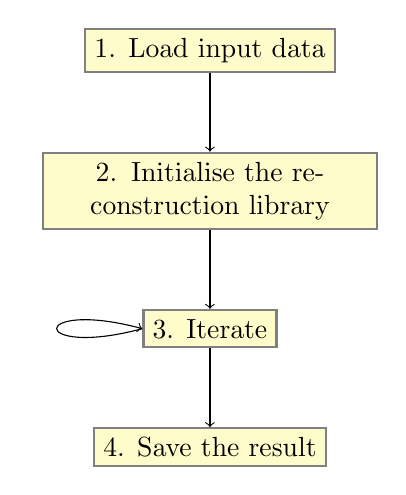
\begin{tikzpicture}[auto,mybox/.style={rectangle,draw=black!50,fill=yellow!20,thick},
      mybox2/.style={rectangle,draw=black!50,fill=blue!20,thick},
      mybox3/.style={rectangle,fill=black!10,minimum height=2cm,minimum width=5cm},
      mybox4/.style={rectangle,fill=white!10,minimum height=7.5cm,minimum width=7.5cm},
      mybox5/.style={rectangle}]
  
    \node[mybox] (load) {1. Load input data};
    \node[mybox] (initialise)   [below=of load,text width=4cm,text centered] {2. Initialise the reconstruction library};
    \node[mybox] (iterate)      [below=of initialise]    {3. Iterate};
    \node[mybox] (result)  [below=of iterate]    {4. Save the result};
              
    \draw [->] (load.south) -- (initialise.north);
    \draw [->] (initialise.south) -- (iterate.north);
    \draw [->] (iterate.west) to [->,loop left,looseness=16,min distance=15mm](iterate.west);
    \draw [->] (iterate.south) -- (result.north);              

  \end{tikzpicture}  
  \end{minipage}
  \caption{\label{fig:reco}The basic steps involved in a CDI reconstruction}
\end{figure}

\begin{enumerate}



\end{comment}


\begin{comment}    
  \begin{scope}[xshift=5.5cm,yshift=-2.5cm]
    
    \node [mybox4] (highlight){};
         
    %      \only<1>{
    \node [mybox2] (intensity) at (-1.5,-0.5) {scale intensity};
    \node [mybox2] (support) [right=of intensity] {apply support};
    
    \draw [->] (intensity.south) to [in=270,out=270] node [auto,swap] {propagate to sample plane}(support.south) ; 
    \draw [<-] (intensity.north) to [in=90,out=90] node [auto] {propagate to detector plane} (support.north) ;
    %      }
    

                  \uncover<2-5>{

                    \node [mybox4] {
                      
                      \begin{minipage}{6cm}
                        
                        \only<2>{
                          Functions are provided for reading hdf, tiff and ppm image
                          files. \\
                          
                          {\bf In C++} 
                          \begin{myverbatim}[language=C++]
                            //read in the data
                            Double_2D data;
                            read_image(``data_file_name.tiff'', data);
                            
                            //read in the support shape
                            Double_2D support;
                            read_image(``support_file_name.tiff'', support);
                          \end{myverbatim}
                          
                          {\bf In IDL}
                          \begin{myverbatim}[language=IDL]
                            data = CXS_READ_PPM(1024, 1024, 'data_file.ppm')
                          \end{myverbatim}
                          etc. or use one of IDLs built in libraries to get
                          the input in matrix form.
                        }
                        
                        \only<3>{
                          The reconstruction code must be initialised for either
                          plane-wave, Fresnel white-field, Fresnel or phase diverse
                          reconstruction. \\
                          
                          {\bf In C++} 
                          \begin{myverbatim}[language=C++]
                            //Create a complex 2D field which will
                            //hold the result of the reconstruction.
                            Complex_2D object_estimate(nx,ny);
                            
                            //Create the planar CDI object which will
                            //be used to perform the reconstruction.
                            PlanarCDI planar(object_estimate);
                            
                            //set the support and intensity
                            planar.set_support(support,false);
                            planar.set_intensity(data);
                          \end{myverbatim}
                              {\bf In IDL}
                              \begin{myverbatim}[language=IDL]
                                CXS_INIT_PLANAR, data, support
                              \end{myverbatim}
                        }
                          
\end{comment}

\subsection{Data Input/Output and Preparation}

\subsubsection{Read Image Files}

\label{subsec:read_images}

The software is capable of accepting data in hdf, tiff or ppm image
format. It can output as a grey scale tiff or ppm image with X bytes
per pixel. In addition data can be read and stored as a binary file of
doubles. This may be useful in situations where high prescision is
required. Similarly, two dimensional arrays of complex numbers, such
as those produced in the reconstruction, may be stored as a binary
file of fftw~\cite{} complex number types.

{\bf In C++} 
\begin{myverbatim}[language=C++]
  //read in the data
  Double_2D data;
  read_image(``data_file_name.tiff'', data);
  
  //read in the support shape
  Double_2D support;
  read_image(``support_file_name.tiff'', support);
  \end{myverbatim}

{\bf In IDL}
\begin{myverbatim}[language=IDL]
   data = CXS_READ_PPM(1024, 1024, 'data_file.ppm')
\end{myverbatim}
etc. or use one of IDLs built in libraries to get
the input in matrix form.


\subsubsection{Write Image Files}
\label{subsub:write_images}
Save the result to file.\\
                          
{\bf In C++} 
\begin{myverbatim}[language=C++]
  //write out the result:
  // - as a complex binary file
  write_cplx(temp_str.str(),object_estimate);
  // - just the magnitude as an image
  Double_2D object_mag;
  object_estimate.get_2d(MAG,object_mag);
  write_image("mag.tiff",object_mag);
\end{myverbatim}
                          
{\bf In IDL}
\begin{myverbatim}[language=IDL]
  ; Record the complex field to a binary file
  CXS_WRITE_CPLX, result, 'result_file.cplx'
\end{myverbatim}
The magnitude and phase of the complex matrix
can be viewed and saved using the standard IDL
routines.


%\subsubsection{Plot the average intensity versus frame number, full-frame and ROI}
%\subsubsection{Check for saturation/dead pixels}
%\subsubsection{Run correlations on data and white-fields}
%\subsubsection{Convert HDF files and extract header info}
\subsubsection{Convert between different file formats}



\subsubsection{Output Data on a Log Scale}

\subsubsection{Subtract the darkfield}
%\subsubsection{Check the beam stability in data over time}
%\subsubsection{Check correlations after dark-field subtraction}

\subsubsection{Merge (add or average) data files together}

\subsubsection{Determine the normalisation of the white-field to data}

\subsubsection{Get the autocorrelation function}


\subsection{Perform Reconstruction}

\subsubsection{Perform Plane-wave, Frensel and Fresnel White-Field Reconstruction}
\label{subsubsec:rec}

Whether it is performed in C++ or IDL, a plane-wave, Frensel and
Fresnel white-field reconstruction consists of the following basic
steps:

\begin{enumerate}

\item {\it Load input data} - Functions are provided for reading and
  writing to various image formats. More information on this step is
  given in Section \ref{subsubsec:read_images}. 
  
\item {\it Initialise the reconstruction library} - Whether you are
  performing plane-wave, Fresnel or Phase-diverse/Ptycographic
  reconstruction, you must initialise the library with a number of
  input: the diffraction and support data, initial estimate, and
  parameters which describe the experimental set-up. Please refer to
  Sections \ref{subsubsec:rec_planar,subsubsec:rec_fresnel,subsubsec:rec_phase_div}
  for specific instructions.
      
\item {\it Iterate} - At this stage the iterative algorithms developed by
  \cite[] are run. In the software library, an iteration can be
  performed simply by calling one function:
      
      {\bf In C++}
      \begin{myverbatim}[language=C++]
        planar.iterate();
      \end{myverbatim}
      
      {\bf In IDL}
      \begin{myverbatim}[language=IDL]
        ; Perform one iteration. The exit-
        ; surface-wave is return to 'result'  
        result = CXS_ITERATE()
        
        ; Perform 50 iterations
        result = CXS_ITERATE(50)
      \end{myverbatim}

      Various aspects of the reconstruction can be controlled, for
      example, the algorithm, the relaxation parameter and the
      shrinkwrap algorithm. How this can be achieve with the software
      is described in this section. 


    \item {\it Save the result} - Refer to Section \ref{subsubsec:write_images}.

\end{enumerate}




\subsubsection{Perform Phase-Diverse/Ptychographic Reconstruction}
\label{subsubsec:rec_phase_div}

\subsubsection{Select the algorithm}

By default plane-wave CDI uses the ... algorithm and Fresnel CDI uses
the ... algorithm. This can be easily changed at any point in the
reconstruction using the method

\begin{myverbatim}
void PlanarCDI::set_algorithm(int alg) 	
\end{myverbatim}
Where the algorithm options are:
\begin{description} 
\item ER - error reduction 
\item BIO - basic input-output 
\item BOO - basic output-output 
\item HIO - hybrid input-output 
\item DM - difference map 
\item SF - solvent-flipping 
\item ASR - averaged successive reflections 
\item HPR - hybrid projection reflection 
\item RAAR - relaxed averaged alternating reflectors
\end{description}

For example, if you have an object of type FresnelCDI called ``fcdi'', and
you wish to change the algorithm to HIO:
\begin{myverbatim}
fcdi.set_algorithm(HIO) 	
\end{myverbatim}

In addition to this extensive list, custom algorithms can be
used. Iterative reconstruction algorithms can be expressed as a
combination of the following 5 operators: , , , and Where is the
support projection and is the intensity projection. These can be
combined to form a basis of 10 vectors (see Harray's review). The
parameters to this method set the coefficient for each of these
vectors. Note: the vector set is linearly dependant.

Please see page 22 of the H.M. Quiney review: TUTORIAL REVIEW,
Coherent diffractive imaging using short wavelength light sources,
Journal of Modern Optics, 2010, DOI: 10.1080/09500340.2010.495459

\begin{myverbatim}
void Planar::set_custom_algorithm (double m1,
double 	m2,
double 	m3,
double 	m4,
double 	m5,
double 	m6,
double 	m7,
double 	m8,
double 	m9,
double 	m10	 
)
\end{myverbatim}
			
Parameters:
m1 	Coefficient to the  term
m2 	Coefficient to the  term
m3 	Coefficient to the  term
m4 	Coefficient to the  term
m5 	Coefficient to the  term
m6 	Coefficient to the  term
m7 	Coefficient to the  term
m8 	Coefficient to the  term
m9 	Coefficient to the  term
m10 	Coefficient to the  term




In IDL, the routine ... can be called to select the algorithm.


\subsubsection{Update the support or use the shrink-wrap algorithm}

\subsubsection{Stop a reconstuction, save the result and restart at the same place}

\subsubsection{Modify the reconstruction algorithm by adding a new constraint}

\subsubsection{Refine the experimental parameters during reconstuction}

\subsubsection{Nominate a beam-stop area in plane-wave reconstruction}



\subsection{Perform a Simulation}





\subsection{Installation Options}

\subsubsection{Select Single or Double Precision}

\subsubsection{Compile the IDL wrapper}

%%%%%%%%%%%%%%%%%%%%%%%%%%%%%%%%%%%%%%%%%%%%%%%%%%%%%%%%%%%%%%%
\newpage

\section{Performance}

In designing the code we have tried to find a good balance between
optimising the speed, reducing the memory used, and keeping the code
modulare and simple to read. There is always room to improve the
performance and we provide the figures below as a benchmark of the
current state of the software in version \ver. These values are
independante of whether C/C++, IDL or the command-line tools are used.

\subsection{Speed}

\begin{table}[h!]
\begin{tabular}[h!]{lcc}
\toprule
   & \multicolumn{2}{c}{Iteration per Second} \\
   & Laptop & Desktop \\
   & Intel U2500 @ 1.20GHz & i7-2600 CPU @ 3.40GHz \\
   & 1.5 GB memory & 8 GB memory\\

\midrule
PlanarCDI (ER) & 3.3  &  16 \\
PlanarCDI (HIO) & 2.7 & 13 \\
FresnelCDI - white field & 2.0 & 7 \\
FresnelCDI & 2.7 & 10 \\
FresnelCDI with Complex Constraints & 1.8 & 7 \\
Phase-Diverse/Ptychography & (X-0.6)/N  & (X-2)/N  \\
\bottomrule
\end{tabular}

\caption{\label{table:speed} Iterations performed per second for a
  1024$\times$1024 pixel reconstruction. For
  phase-diverse/ptychography reconstruction, X is the number of
  iterations which could be perform for a single frame,
  non-phase-diverse/ptychography reconstruction of that type
  (i.e. from the first five rows of the table). The start-up time is a
  few seconds in each case. }
\end{table}

\subsection{Memory}

By default the fast fourier transform library used with \name is
single precision. We found no noticible lose in performance or
correctness by using single precision, however users may choose to use
double precision fast fourier transforms by adding the flag
``--enable-double-precision'' to ``./configure'' during installation.
The class Double\_2D, despite its name, will also use the same
precision as the fourier transform library and is single precision by
default.

\begin{table}[h!]
\begin{tabular}[h!]{lcc}
\toprule
&  Number of N$\times$N & With p=4, N=1024 \\
&  pixel arrays used & (MB) \\
\midrule
PlanarCDI (ER) & 4 & 17 \\
PlanarCDI (HIO) & 10 & 42  \\
FresnelCDI - white field & 4.5 & 19 \\
FresnelCDI & 8.5 & 36 \\
FresnelCDI with complex constraints & 11.5+c & 57 (c=2) \\
Phase-Diverse/Ptychography & I(1+X) + 2R & 30,000 (I=400,M = 1100$^2$, \\
 &                 & X = FresnelCDI)  \\
\bottomrule
\end{tabular}

\caption{\label{table:memory}The memory used. 
In total the memory used will be the factor given in the second
coloumn of Figure \ref{table:memory} multiplied by pN$^2$.
(N - image side length in pixels, p - precision in bytes, 
c - number of complex constraint regions, I - number of images, 
R - ratio of the total phase-diverse image size to a single N$\times$N image,
X - number of arrays needed for a single reconstruction). 
}
\end{table}


%%%%%%%%%%%%%%%%%%%%%%%%%%%%%%%%%%%%%%%%%%%%%%%%%%%%%%%%%%%%%%%%%%%%%%
\newpage

\section{Directory Structure}

\begin{itemize}
   \item[] {\tt cxs\_software/} ...... base directory, where ./configure and make should be executed from.
   \begin{itemize}
      \item[] {\tt bin/} ...... contains the command-line tool executable files after compilation.
      \item[] {\tt doc/} ...... contains configuration files for doxygen.
      \begin{itemize}
         \item[] {\tt manual/} ...... contains the latex source for the software manual (this file).
      \end{itemize}
      \item[] {\tt examples/} ...... this directory stores all the examples.
      \begin{itemize}
         \item[] {\tt image\_files/} ...... stores images and data files used in the examples.
      \end{itemize}
      \item[] {\tt include/ }...... contains the source header files after compilation.
      \item[] {\tt interfaces/} ...... a directory for wrapper code to languages other than C/C++.
      \begin{itemize}
         \item[] {\tt idl/} ...... contains all IDL related code (source and examples).
      \end{itemize}
      \item[] {\tt lib/} ...... contains the static and dynamic C++ library after compilation.
      \item[] {\tt src/} ...... a directory for the library source code.
      \item[] {\tt tools/} ...... contains the source code for the command-line tools.
   \end{itemize}
\end{itemize}


%{
%\section{Directory Structure}

%\dirtree{% 
%.1 cxs\_software/\DTcomment{base directory, where ./configure and make should be executed from}.
%.2 bin/ \DTcomment{contains the tool executable files are compilation}.
%.2 doc/ \DTcomment{contains configuration files for doxygen}.
%.3 manual/\DTcomment{contains the latex source for the software manual (this file)}.
%.2 examples/\DTcomment{this directory stores all the examples}.
%.3 image\_files/\DTcomment{stores images and data files used in the examples}.
%.2 include/\DTcomment{contains the source header files after compilation}.
%.2 interfaces/\DTcomment{a directory for wrapper code to languages other than C/C++}.
%.3 idl/\DTcomment{contains all IDL related code (source and examples)}.
%.2 lib/\DTcomment{contains the static and dynamic C++ library after compilation}.
%.2 src/\DTcomment{a directory for the library source code}.
%.2 tools/\DTcomment{contains the source code for the command-line tools}.
%}
%}
%{

%%%%%%%%%%%%%%%%%%%%%%%%%%%%%%%%%%%%%%%%%%%%%%%%%%%%%%%%%%%%%
\newpage

\appendix

\section{C++ Class Description} 

For the sake of advanced users we provide a description of the
software library structure in this section. Figure
\ref{fig:class_diagram} shows the relationship between the non-I/O
class of the software, and lists the public member functions.

The reconstruction classes PlanarCDI, FresnelCDI and FresnelCDI\_WF
(shows in the shaded region of Figure \ref{fig:class_diagram}, all
inherit from the abstract base class, BaseCDI. Common functionality,
for example the definition of the reconstruction algorithms is
provided in BaseCDI. The reconstruction type PhaseDiverseCDI, which is
capable of performing phase-diverse and ptycographic reconstruction
accepts multiple objects of type BaseCDI.



\begin{figure}[htbp]
\centering \includegraphics*[scale=0.32,viewport = 0 0 1500
  1200]{cxs_class_diagram.eps}
\caption[]{The relationship between classes of the \name package.
\label{fig:class_diagram}}
\end{figure}

\subsection{BaseCDI}
The fundamental class used for performing CDI reconstruction; an
object of type "BaseCDI" allows planar CDI to be performed, and it is
also used by the Fresnel reconstruction code (through inheritance).
The reconstruction can be performed in the following way:

\begin{itemize}

\item The user should create an object to store the result (the exit
  surface wave of type Complex\_2D). For example using: Complex\_2D
  esw\_estimate(nx,ny) This can be initialise to a best guess, or can
  be left for the BaseCDI object to initialise.

\item The BaseCDI object should be created and the Complex\_2D
  previously created should be passed as input. For example: BaseCDI
  my\_planar\_recon(esw\_estimate)

\item The support and intensity data should be set, and the exit
  surface wave initialised to a first guess (if not already done):
  \begin{myverbatim}
my_planar_recon.set_support(support) 
my_planar_recon.set_intensity(data) 
my_planar_recon.initialise_estimate()
\end{myverbatim}

\item The reconstruction can be configured before, or at anytime
  during the reconstruction using setter methods. For example the
  algorithm choice and relaxation parameters:
\begin{myverbatim}
my_planar_recon.set_algorithm(HIO) 
my_planar_recon.set_relaxation_parameter(0.95) 
\end{myverbatim}
The algorithm is fully customisable through the
BaseCDI::set\_custom\_algorithm method. See page 22 of the H.M. Quiney
review: TUTORIAL REVIEW, Coherent diffractive imaging using short
wavelength light sources, Journal of Modern Optics, 2010, DOI:
10.1080/09500340.2010.495459 for the formalism.

\item The reconstruction is then performed with multiple calls to the
  BaseCDI::iterate() method:
\begin{myverbatim}
my_planar_recon.iterate() 
\end{myverbatim}
This will automatically update the values in the Complex\_2D estimate
and the current error. The error can be retrieved using
BaseCDI::get\_current\_error().
\end{itemize}

For cases where the beam-stop region must be excluded during
reconstruction, you should call the set\_beam\_stop() method, to define
the beam-stop region before running iterate().


\subsection{PlanarCDI}

\subsection{FresnelCDI}
The class used for performing Fresnel CDI reconstruction (for
white-field reconstruction see FresnelCDI\_WF). It inherits most
methods from BaseCDI, so please look at the documentation of this
class also. Although there are some differences in the underlying code
between this class and the planar case, the interface is generally
unchanged. Therefore users should refer to the instructions for
BaseCDI to understand how to use a FresnelCDI object in their own
code. Only the differences relevant to users will be documented here.

\subsection{FresnelCDI\_WF}
This is the class used for reconstructing white-field data prior to
running Fresnel reconstruction with FresnelCDI. It inherits most
methods from BaseCDI, so please look at the documentation of this
class also. Although there are some differences in the underlying code
between this class and the planar case, the interface is generally
unchanged. Therefore users should refer to the instructions for
BaseCDI to understand how to use a FresnelCDI\_WF object in their own
code. Only the differences relevant to users will be documented here.

\subsection{PhaseDiverseCDI}

This class can be used to perform phase diverse or ptychographic
reconstruction of either Fresnel or plane-wave CDI data. Any number of
frames (also called local/single frames or probes in this
documentation) may be added to the reconstruction. In order to perform
a reconstruction, you will need to create either a new FresnelCDI or
PlanarCDI object for each of these 'local' datasets. The FresnelCDI or
PlanarCDI objects must then be passed to a PhaseDiverseCDI
object. Because the each sub-iteration (ie. each iteration of a local
frame) is performed using the code in FresnelCDI/PlanarCDI, all the
functionality available in these classes is also available here. For
example complex constraint can be set, shrink-wrap can be used, the
estimate can be initialised using the results from a previous
reconstruction etc. An example can be found in the /examples
directory, demonstrating how to use PhaseDiverseCDI.

The displacement in position between 'local' frames may be either
transverse to the beam direction, or longitudinal, along the beam
direction. The longitudinal position (for FresnelCDI) is set when the
FresnelCDI objects are initially constructed. Transverse positions are
set when the FresnelCDI/PlanarCDI objects are added to the
PhaseDiverseCDI object. This class allows the transverse positions to
be automatically adjusted during reconstruction using the
"adjust\_positions" function.

The code allows for several options in the type of reconstruction
which is done:

\begin{itemize}

\item The reconstruction can be performed in series or parallel.
  \begin{itemize}

    \item In the case of series (see for example the paper....), a
      'local' frame will undergo one or more iterations, the result
      will be updated to a 'global' estimate of the sample, and this
      estimate will form the starting point for the next frame. For
      each call to the method "iterate()" this process is repeated
      until each local frame is used once. The algorithm can be
      described by:
      \[ T_{k+1} = (1-\beta w^n)T_k + \beta w^n T^n_k \] 
      where $T_{k+1}$ is the updated global function, $T^n$ is the
      updated local function for the nth local frame. $\beta$ is the
      relaxation parameter and the weight is $ w^n(\rho) = \alpha^n
      (\frac{|T^n(\rho)|}{max|T^n(\rho)|} )^\gamma $ for Fresnel CDI
      or $w^n = \alpha^n$ for Plane-wave CDI. The weight is zero
      outside of the support.

   \item For a parallel reconstruction (see .....), each frame with
     independently undergo one of more iteration, the result from all
     frames will be merged to form a new estimate of the sample, this
     estimate then becomes the starting point for the next iteration
     of all frames. The algorithm can be described by:
     \[T_{k+1} = (1-\beta)T_k + \beta \sum_n(w^n T^n_k)\]
     where $T_{k+1}$, $T^n$, and $\beta$ were defined
    earlier. The weight, w, is similar to that used for series
    reconstruction, but the weight it normalised such that 
    $ \sum_n w^n = 1 $.  i.e. $ w^n_{parallel}= w^n_{series} / \sum_n w^n_{series} $

\end{itemize}

\item The number of local iterations to perform before updating the
  result to the 'global' function can be set.

\item The feedback parameter, beta, may be set. This quantity is used
  to set how much of the previous 'global' sample function will be
  left after the next 'global' iteration.

\item The amplification factor, gamma, and the probe scaling, alpha,
  may also be see. These parameters control the weighting of one frame
  (and pixels within a frame) with respect to each other.

\end{itemize}

\subsection{TransmissionConstraint}
This class allows constraints on the transmission function
(FresnelCDI) or exit-surface-wave (PlanarCDI), such as complex
constraints to be used. To achieve this the user needs to: create an
instance of this class configure it (for example by setting some
ComplexConstraint objects and finally by passing this object to the
reconstruction (through the PlanarCDI or FresnelCDI function
"set\_complex\_constraint").

\subsection{ComplexConstraint}

This class is based on the paper "Use of a complex constraint in
coherent diffractive imaging", J. N. Clark et. al., 2010. The notation
used there is also used here. Users should have knowledge of this or
similar papers before using this class.

A section of the reconstructed transmission function will be updated
according to a restriction on the value of c (c = beta/delta). If the
material is of a known element, then c can be fixed to the know value,
and the phase and magnitude of the transmission function updated
accordingly. Alternatively, c can be left to float, and calculated for
each iteration from a mean over the defined region. The parameters
alpha1 and alpha2 are used to control the strength of the constraint.

Instances of this class should be pass to a TransmissionConstraint
object. If a sample consists of different regions which are locally
homogeneous in element, multiple instances of this class should be
created, each one defining a different region of the sample, and then
each should be added to the TransmissionConstraint object.

\subsection{Double\_2D}
This class represents a 2D field of doubles. Setter and getter methods
are provided along with some other useful functions. This is a
convenient form to store and pass image data in the reconstruction
software. A better implementation of this class would use templates,
but restricting the type to double is sufficient our needs.

\subsection{Complex\_2D}
This class represents a 2D complex field. Setter and getter methods
are provided along with some other useful functions (add, multiplying
and fast fourier transforming). Complex\_2D objects are used in the CDI
reconstruction to represent the ESW in a single plane.

\subsection{Config}
This class allows simple text files to be read and is used by the
command line tool programs. The parser takes a file name and
constructs key-value pairs for each line with the syntax:\\ 
key = value or \\
key = value\_1 value\_2 value\_3 ... \\
White spaces are ignored and everything to the right of a "\#" symbol
is also ignored (this allows comments to be included in the config
file. See example.config to see how it looks. If a key (as given by
any of the methods below) is not found in the file, the status is set
to FAILURE and the method returns either 0, an empty string or list.

%%%%%%%%%%%%%%%%%%%%%%%%%%%%%%%%%%%%%%%%%%%%%%%%%%%%%%%%%%%%%%

\section{IDL Routine Descriptions}
\label{sec:idl_routines}
The complete list of IDL routines provided with release 0.4 of the
DIXE software is described below. This documentation can also be found
on the project website and will be updated with new releases of the
software.



\subsection{NADIA\_ADD\_COMPLEX\_CONSTRAINT\_REGION}
\begin{verbatim}

 NAME:
       NADIA_ADD_COMPLEX_CONSTRAINT_REGION

 PURPOSE: For use with FresnelCDI reconstruction. Calling this
       procedure will constrain the transmission function magnitude
       and phase using the method from the paper "Use of a complex
       constraint in coherent diffractive imaging", J. N. Clark
       et. al., 2010. The notation used there is also used
       here. Users should have knowledge of this or similar papers
       before using the procedure.

       A section of the reconstructed transmission function will be
       updated according to a restriction on the value of c (c =
       beta/delta). If the material is of a known element, then c can
       be fixed to the know value, and the phase and magnitude of the
       transmission function updated accordingly. Alternatively, c
       can be left to float, and calculated for each iteration from a
       mean over the defined region. The parameters alpha1 and alpha2
       are used to control the strength of the constraint. This
       procedure should be called once before each region of
       homogenious material.

 CALLING SEQUENCE:

       NADIA_ADD_COMPLEX_CONSTRAINT_REGION, region, alpha1, alpha2 [, fixed_c]

 INPUTS:

       region:
             A 2 array of doubles which is used to indicate which
             pixels the constraint should be applied to. 0 -
             indicated the array element does not belong to the
             region. Any other value indicated that it does.

       alpha1:
             Constraint strength parameter for the amplitude (double
             type).

       alpha2:
             Constraint strength parameter for the phase (double
             type).
             
       fixed_c:
             Optional parameter to fix the value of c = beta/delta
             (double type).

 EXAMPLE:
       Setting a complex constraint for two image regions.
       For the second, the value of c=beta/delta is fixed.

       r1 =  nadia_read_tiff(1024,1024,'region_1.tiff')
       r2 =  nadia_read_tiff(1024,1024,'region_2.tiff')

       delta = 6.45e-4;
       beta = 1.43e-4;

       nadia_add_complex_constraint_region, r1, 0.5, 0.5
       nadia_add_complex_constraint_region, r2,   1,   0, beta/delta

\end{verbatim}



  
 
\subsection{NADIA\_APPLY\_SHRINKWRAP}
\begin{verbatim}

 NAME:
       NADIA_APPLY_SHRINKWRAP

 PURPOSE:
       Apply the shrinkwrap algorithm. The current exit-surface-wave
       magnitude is used to update the support; it is convoluted with
       a Gaussian and then a threshold is applied. You can use the
       nadia_get_support function to see how the support have been
       modified after calling this procedure.

 CALLING SEQUENCE:

	NADIA_APPLY_SHRINKWRAP [,gauss_width, threshold ]

 INPUTS:

       gauss_width: 
             The width (1-standard deviation. in pixels) of the Gaussian
             used for smearing. If this parameter is not passed, 
             a width of 1.5 pixels is used.

       threshold:
             All pixels which are below the threshold are set to zero 
             (outside the support). The threshold should be given as
             a fraction of the maximum pixel value (in double format). 
             If this parameter is not passed a threshold of 0.1 (10%)
             is used.

 EXAMPLE:
       Perform 1000 iterations in total, applying shrink-wrap at the 400th iteration:

       ....
       a = NADIA_ITERATE(400)
       NADIA_APPLY_SHRINKWRAP
       a = NADIA_ITERATE(600)

\end{verbatim}


\subsection{NADIA\_APPLY\_SUPPORT}
\begin{verbatim}

 NAME:
       NADIA_APPLY_SUPPORT

 PURPOSE:
       Apply the support constraint to the given complex array. All
       elements outside the support with be reset to zero. Elements
       within the support will be left as they are. The support must
       have been previously set using either one of the NADIA_INIT 
       functions or NADIA_SET_SUPPORT.

       This function is called when using (NADIA_ITERATE) so generally
       won't need to be call explicitly. An exception to this is if
       the user wishes to extend their reconstruction with an
       addition constraint.


 CALLING SEQUENCE:

	result = NADIA_APPLY_SUPPORT( complex_array [,/SUPPRESS_DISPLAY] )

 INPUTS:

       complex_array:
             A 2D array of COMPLEX values which represents a wave in
             either the sample plane (for planar and Fresnel
             reconstruction) or the zone-plate plane for Fresnel 
             white-field reconstruction.

 KEYWORD PARAMETERS:

       /SUPPRESS_DISPLAY:
             Do not display the result on the screen. This maybe useful
             if this function is used within a for loop. 

 OUTPUTS:

       result:
             A COMPLEX 2D array after the support is applied.

 EXAMPLE:
       See the example for NADIA_PROPAGATE_FROM_DETECTOR

\end{verbatim}




\subsection{NADIA\_CLEAR\_MEMORY}
\begin{verbatim}

 NAME:
       NADIA_CLEAR_MEMORY

 PURPOSE:
       Clean-up after a reconstruction has been performed. This 
       procedure should be called at the very end of a program.
       It will free up the memory that was allocated when one of 
       the "NADIA_INIT_.." methods was called.

 CALLING SEQUENCE:

       NADIA_CLEAR_MEMORY

 EXAMPLE:
       NADIA_CLEAR_MEMORY

\end{verbatim}

\subsection{NADIA\_GET\_BEST\_RESULT}
\begin{verbatim}

 NAME:
       NADIA_GET_BEST_RESULT

 PURPOSE:
       Get the best (lowest error) result found during the reconstruction.
       The result is returned and the magnitude of the result is
       displayed as a 512x512 pixel image on the screen.

 CALLING SEQUENCE:

       result = NADIA_GET_BEST_RESULT()

 OUTPUTS:

       result:
             A 2D array of COMPLEX variables. For planar and Fresnel
             reconstruction this will be the  exit-surface-wave for
             the sample. For Fresnel white-field reconstruction, this
             will be the complex white-field in the detector plane.


 EXAMPLE:
       Perform 1000 iterations and get the lowest error result.
       ....
       a = NADIA_ITERATE(1000)
       a = NADIA_GET_BEST_RESULT()

\end{verbatim}

\subsection{NADIA\_GET\_ERROR}
\begin{verbatim}

 NAME:
       NADIA_GET_ERROR

 PURPOSE:
       Get the error metric. This is defined as the difference
       between the estimated diffraction and the actual diffraction
       pattern and is calculated as:
           sum over pixels of ( M - sqrt(I) ) ^2 / sum(I) 
       Where I is the detector data and M is the magnitude of the
       estimate in the detector plane. Note that due to the way this
       quantity is calculated, it actually corresponds to the
       previous estimate rather than the current iteration.


 CALLING SEQUENCE:

       error = NADIA_GET_ERROR()

 OUTPUTS:

       error:
             The error. 

 EXAMPLE:

       a = NADIA_GET_ERROR()

\end{verbatim}

 
\subsection{NADIA\_GET\_INTENSITY\_AUTOCORRELATION}
\begin{verbatim}

 NAME:
       NADIA_GET_INTENSITY_AUTOCORRELATION

 PURPOSE:
       Get the autocorrelation function from the intensity data.
       This method is only useful for planar CDI reconstruction.

 CALLING SEQUENCE:

       a = NADIA_GET_INTENSITY_AUTOCORRELATION()

 OUTPUTS:
       a:
             The autocorrelation function (a 2D array of doubles).

 EXAMPLE:
       a = NADIA_GET_INTENSITY_AUTOCORRELATION()

\end{verbatim}

\subsection{NADIA\_GET\_ROUND\_SUPPORT}
\begin{verbatim}

 NAME:
       NADIA_GET_ROUND_SUPPORT

 PURPOSE: 
       This function will return a simple array with a central
       circular region where each element has the value 1.0. Outside
       the value returned is zero. This function has been written to
       allow each create of the support array. For example when
       reconstructing the white-field for Fresnel CDI reconstruction.
       Note that it does not actually call any method from the NADIA
       software library.

 CALLING SEQUENCE:

	NADIA_GET_ROUND_SUPPORT, nx, ny, radius

 INPUTS:

       n_x: 
             The number of pixels in the horizontal direction of the
             output array.
       n_y: 
             The number of pixels in the vertical direction of the
             output array.
       radius: 
             The radius of the circle in pixels.

 RETURN:
       A two dimensional array which can be used to set the support
       for any of the CDI reconstructions.

 EXAMPLE:

       nadia_get_round_support, 1024, 1024, 0.25*1024

\end{verbatim}

 
\subsection{NADIA\_GET\_SUPPORT}
\begin{verbatim}

 NAME:
       NADIA_GET_SUPPORT

 PURPOSE:
       Get the support. This maybe useful to see how shrinkwrap has
       effected the support. The result is displayed as a 512x512 
       pixel image on the screen.

 CALLING SEQUENCE:

       support = NADIA_GET_SUPPORT()

 OUTPUTS:

       support:
             The support. A 2D array of doubles. A pixel with value below 1
             is outside the support and 1 and above is inside the support.

 EXAMPLE:
       View the support after applying shrink-wrap.
 
       NADIA_APPLY_SHRINKWRAP
       a = NADIA_GET_SUPPORT()

\end{verbatim}

\subsection{NADIA\_GET\_TRANSMISSION\_FUNCTION}
\begin{verbatim}

 NAME:
       NADIA_GET_TRANSMISSION_FUNCTION

 PURPOSE:
       Get the transmission function from the current estimate of the
       exit-surface-wave. The magnitude of the result will be
       displayed on the screen. Note that this functions
       is only available for Fresnel CDI reconstruction.

 CALLING SEQUENCE:

       result = NADIA_GET_TRANSMISSION_FUNCTION()

 OUTPUTS:

       result:
             The transmission function for the sample. A 2D array of
             COMPLEX variables is returned. 

 EXAMPLE:
       a = NADIA_GET_TRANSMISSION_FUNCTION()

\end{verbatim}

 
\subsection{NADIA\_INITIALISE\_ESW}
\begin{verbatim}

 NAME:
       NADIA_INITIALISE_ESW

 PURPOSE:
       Initialise the exit-surface-wave guess. The initialisation
       will depend on the reconstruction type (see the procedures
       which begin "NADIA_INIT_" for a description). The "INIT" procedure  
       will call this procedure if no starting guess is provided. 
       It is useful if you wish to run the same reconstruction
       several time with a different random starting point, or if 
       you wish to reset the reconstruction back to the original guess.


 CALLING SEQUENCE:

	NADIA_INITIALISE_ESW, seed

 INPUTS:

       seed: 
             Seed for the random number generator used to initialise
             the guess. It should be an integer. This is ignored in 
             the case of Fresnel CDI.


 EXAMPLE:

       nadia_initialise_esw, 6

\end{verbatim}


\subsection{NADIA\_INIT\_FRESNEL}
\begin{verbatim}

 NAME:
       NADIA_INIT_FRESNEL

 PURPOSE:
       Set-up a Fresnel CDI reconstruction. This will
       initialise the reconstruction using a previously reconstructed
       white-field, detector data, sample support and experimental 
       parameters. Some defaults will be set and memory will be
       allocated ready for reconstructing the sample
       exit-surface-wave. It is necessary to call this procedure before
       attempting to call any of the reconstruction methods
       (e.g. before setting the algorithm or calling NADIA_ITERATE).

       Calling this procedure will initialise the reconstruction algorithm
       to the error-reduction with a relaxation parameter of 0.9.

 CALLING SEQUENCE:

	NADIA_INIT_FRESNEL, data, support, white-field, beam_wavelength,
	                  focal_detector_length, focal_sample_length, 
                         pixel_size [, normalisation, starting_point ]

 INPUTS:

       You may use any length units for the experimental parameters
       below, as long as all quantities are given in the same units.

	data: 
             The detector data with the sample in place. It should be
             in the form of a 2D array.

       support: 
             A 2D array of integers or doubles which give the sample support.
             Values or 1 or greater are considered inside
             the support. All others are considered to be
             outside the support.

       white-field:
             A COMPLEX 2D array of the reconstructed white-field in
             the detector plane. This can be recovered using 
             NADIA_INIT_FRESNEL_WF followed by NADIA_ITERATE.

       beam_wavelength:
             The beam wavelength.

       focal_detector_length:
             The distance between the focal point and the detector.

       focal_sample_length:
             The distance between the focal point and the sample.

       pixel_size:
             The side length of one detector pixel.

       normalisation: 
             The factor to scale the white-field before
             performing FCDI. If this parameter is excluded, the
             ratio of the square-root of the intensity data and the
             white-field magnitude is used as the normalisation.

       starting_point: 
             As an option you may supply an initial 
             guess of the exit-surface-wave for the sample. 
             This maybe useful, for example, if you wish to 
             start from the end point of a previous run. The
             format of this parameter much be a 2D array of
             COMPLEX variables. If this parameter is not supplied,
             the initialisation described in Harry's review paper: 
             page 29. (in particular e.q. 137) is used.

 EXAMPLE:

        nadia_init_fresnel, my_data, my_supports, my_white-field, $
                          4.892e-10, 0.9078777, 2.16e-3, $
                          13.5e-6

\end{verbatim}

\subsection{NADIA\_INIT\_FRESNEL\_WF}
\begin{verbatim}

 NAME:
       NADIA_INIT_FRESNEL_WF

 PURPOSE:
       Set-up a Fresnel white-field CDI reconstruction. This will
       initialise the reconstruction with the white-field intensity, 
       zone-plate support and experimental parameters. Some defaults 
       will be set and memory will be allocated ready for 
       reconstructing the white-field (phase and magnitude) in the
       detector plane. It is necessary to call this procedure before
       attempting to call any of the reconstruction methods
       (e.g. before setting the algorithm or calling NADIA_ITERATE).

 CALLING SEQUENCE:

	NADIA_INIT_FRESNEL_WF, data, support, beam_wavelength,
                            zone_focal_length, focal_detector_length,
                            pixel_size [,starting_point]

 INPUTS:

       You may use any length units for the experimental parameters
       below, as long as all quantities are given in the same units.

	data: 
             The white-field illumination. It should be
             in the form of a 2D array.

       support: 
             A 2D array of integers or doubles giving the zone-plate support.
             Values or 1 or greater are considered inside
             the support. All others are considered to be
             outside the support.

       beam_wavelength:
             The beam wavelength.

       zone_focal_length:
             The distance between the zone plate and the focal point.

       focal_detector_length:
             The distance between the focal point and the detector.

       pixel_size:
             The side length of one detector pixel.

       starting_point: 
             As an option you may supply an initial guess of the 
             white-field. This may be useful, for example, if you 
             wish to start from the end point of a previous run. The
             format of this parameter must be a 2D array of
             COMPLEX variables. If this parameter is not supplied,
             the starting point is initialised to be zero outside
             the support, a random number inside the support 
             for the magnitude and zero for the phase.

 EXAMPLE:

        An example of loading two 2D arrays from file and using
        them to initialise the white-field reconstruction for FCDI:

        my_support = nadia_read_tiff(1024,1024,'support.tiff')
        my_data = nadia_read_tiff(1024,1024,'data.tiff')
        nadia_init_fresnel_wf, my_data, my_support, $
                   4.892e-10, 16.353e-3, 0.9078777,13.5e-6

\end{verbatim}

\subsection{NADIA\_INIT\_PLANAR}
\begin{verbatim}

 NAME:
       NADIA_INIT_PLANAR

 PURPOSE:
       Set-up a planar CDI reconstruction. This will
       initialise the reconstruction with the data
       and support. Some defaults will be set and
       memory will be allocated ready for reconstruction.
       It is necessary to call this procedure before
       attempting to call any of the reconstruction methods
       (e.g. before setting the algorithm or 
       calling NADIA_ITERATE).

       Calling this procedure will initialise the reconstruction 
       algorithm to hybrid-input-output with a relaxation parameter of 0.9.


 CALLING SEQUENCE:

	NADIA_INIT_PLANAR, Data, Support [,Starting_point]


 INPUTS:

	Data: 
             The detector illumination. It should be
             in the form of a 2D array

       Support: 
             A 2D Array giving the sample support.
             Values or 1 or greater are considered inside
             the support. All others are considered to be
             outside the support.

       Starting_point: 
             As an option you may supply an initial 
             guess of the exit-surface-wave for the sample. 
             This maybe useful, for example, if you wish to 
             start from the end point of a previous run. The
             format of this parameter much be a 2D array of
             COMPLEX variables. If this parameter is not supplied,
             the starting point is initialised to be zero outside
             the support and a random number inside the support, 
             for both the magnitude and phase.

 EXAMPLE:
        An example of loading two 2D arrays from file and using
        them to initialise the planar reconstruction:

        my_support = nadia_read_tiff(1024,1024,'planar_support.tiff')
        my_data = nadia_read_tiff(1024,1024,'planar_data.tiff')
        NADIA_INIT_PLANAR, my_data, my_support


\end{verbatim}






  
 
\subsection{NADIA\_ITERATE}
\begin{verbatim}

 NAME:
       NADIA_ITERATE

 PURPOSE:
       Perform the iterative reconstruction. The number of iterations
       to perform should be given and the result of the final
       iteration is returned. For planar and Fresnel CDI this will be
       the exit surface wave of the sample. For Fresnel white-field
       reconstruction it will be the white-field at the detector surface.
       The magnitude of the result is also displayed on the screen as
       a 512x512 pixel image. The iteration number and corresponding
       error (see NADIA_GET_ERROR) will be printed on the screen.

       NADIA_ITERATE may be called several time and the reconstruction
       will start from where is ended. i.e. calling NADIA_ITERATE(50),
       followed by a second NADIA_ITERATE(50) is equivalent to calling
       NADIA_ITERATE(100).

       During the reconstruction, the best (lowest error) result is
       also stored. It maybe retrieved by calling NADIA_GET_BEST_RESULT.
 

 CALLING SEQUENCE:

	result = NADIA_ITERATE([iterations])

 INPUTS:

       iterations: 
             The number of iterations to perform (an integer). 
             If left empty, one iteration is performed.

 OUTPUTS:

       result:
             A COMPLEX 2D array. For planar and Fresnel CDI this will be
             the exit surface wave of the sample. For Fresnel white-field
             reconstruction it will be the white-field at the detector surface.


 EXAMPLE:

       my_result = nadia_iterate(100)

\end{verbatim}






  
 
\subsection{NADIA\_PRINT\_ALGORITHM}
\begin{verbatim}

 NAME:
       NADIA_PRINT_ALGORITHM

 PURPOSE:
       Output the form of the current algorithm to the screen. 
       It will be written in terms of the support and intensity
       projection operators.


 CALLING SEQUENCE:
       NADIA_PRINT_ALGORITHM


 EXAMPLE:
       NADIA_SET_ALGORITHM, 'RAAR'
       NADIA_PRINT_ALGORITHM

\end{verbatim}



  
 
\subsection{NADIA\_PROPAGATE\_FROM\_DETECTOR}
\begin{verbatim}

 NAME:
       NADIA_PROPAGATE_FROM_DETECTOR

 PURPOSE:
       Propagate the given wave field from the detector plane to the 
       sample plane (planar and Fresnel) or zone-plate plane (Fresnel
       white-field reconstruction). The result will be returned and
       displayed on the screen by default.

       This function is called when using (NADIA_ITERATE) so generally
       won't need to be call explicitly. An exception to this is if
       the user wishes to extend the reconstruction with an addition
       constraint (see the example below).


 CALLING SEQUENCE:

	result = NADIA_PROPAGATE_FROM_DETECTOR( complex_array [,/SUPPRESS_DISPLAY] )

 INPUTS:

       complex_array:
             A 2D array of COMPLEX values which represents a wave in
             the detector plane.

 KEYWORD PARAMETERS:

       /SUPPRESS_DISPLAY:
             Do not display the result on the screen. This maybe useful
             if this function is used within a for loop. 

 OUTPUTS:

       result:
             A COMPLEX 2D array which is either the field in the
             sample plane (for planar and Fresnel reconstruction) or
             the zone-plate plane for Fresnel white-field reconstruction.

 EXAMPLE:
       Performing the reconstruction with a new constraint applied in the
       sample plane (e.g. called "NEW_SUPPORT"):

              FOR K = 0, 100 DO BEGIN 
                  a = NADIA_PROPAGATE_TO_DETECTOR(a,/SUPPRESS_DISPLAY)
                  a = NADIA_SCALE_INTENSITY(a,/SUPPRESS_DISPLAY)
                  a = NADIA_PROPAGATE_FROM_DETECTOR(a,/SUPPRESS_DISPLAY)
                  a = NADIA_APPLY_SUPPORT(a,/SUPPRESS_DISPLAY)
                  a = NEW_SUPPORT(a)
              ENDFOR 


\end{verbatim}






  
 
\subsection{NADIA\_PROPAGATE\_TO\_DETECTOR}
\begin{verbatim}

 NAME:
       NADIA_PROPAGATE_TO_DETECTOR

 PURPOSE:
       Propagate the given wave field to the detector plane from the 
       sample plane (planar and Fresnel) or zone-plate plane (Fresnel
       white-field reconstruction). The result will be returned and
       displayed on the screen by default.

       This function is called when using (NADIA_ITERATE) so generally
       won't need to be call explicitly. An exception to this is if
       the user wishes to perform simulation or to extend their
       reconstruction with an addition constraint (see the previous
       example).


 CALLING SEQUENCE:

	result = NADIA_PROPAGATE_TO_DETECTOR( complex_array [,/SUPPRESS_DISPLAY] )

 INPUTS:

       complex_array:
             A 2D array of COMPLEX values which represents a wave in
             either the sample plane (for planar and Fresnel
             reconstruction) or the zone-plate plane for Fresnel 
             white-field reconstruction.

 KEYWORD PARAMETERS:

       /SUPPRESS_DISPLAY:
             Do not display the result on the screen. This maybe useful
             if this function is used within a for loop. 

 OUTPUTS:

       result:
             A COMPLEX 2D array which is the field in the detector plane.

 EXAMPLE:
       Performing Fresnel simulation (assuming you already have a
       complex white-field called "white_field" and the transmission
       function of the object, "trans").

       white_field_at_sample = NADIA_PROPAGATE_FROM_DETECTOR(white_field)
       esw_at_sample = trans*white_field_at_sample
       esw_at_detector = NADIA_PROPAGATE_TO_DETECTOR(esw_at_sample)
       diffraction_pattern = abs(esw_at_detector)^2

\end{verbatim}






  
 
\subsection{NADIA\_READ\_CPLX}
\begin{verbatim}

 NAME:
       NADIA_READ_CPLX

 PURPOSE:
       Read a binary file of fftw complex numbers. This is
       useful for storing and restoring the result of a reconstruction.

 CALLING SEQUENCE:

       complex_array = NADIA_READ_CPLX( nx, ny, filename)

 INPUTS:

       nx:
             The number of pixels horizontally (need to be checked?)

       ny:
             The number of pixels vertically (need to be checked?)

       filename:
             A string containing the name of the file to read.

 OUTPUTS:
       complex_array:
             A 2D array of COMPLEX numbers.

 EXAMPLE:
       white_field = NADIA_READ_CPLX(1024, 1024, 'white_field_file.cplx')

\end{verbatim}






  
 
\subsection{NADIA\_READ\_DBIN}
\begin{verbatim}

 NAME:
       NADIA_READ_DBIN

 PURPOSE:
       Read a double binary file (a binary file of doubles).

 CALLING SEQUENCE:

       image = NADIA_READ_DBIN( nx, ny, filename)

 INPUTS:

       nx:
             The number of pixels horizontally (need to be checked?)

       ny:
             The number of pixels vertically (need to be checked?)

       filename:
             A string containing the name of the file to read.

 OUTPUTS:
       image:
             The image in the format of a 2D array of doubles.

 EXAMPLE:
       data = NADIA_READ_DBIN(1024, 1024, 'data_file.dbin')

\end{verbatim}






  
 
\subsection{NADIA\_READ\_PPM}
\begin{verbatim}

 NAME:
       NADIA_READ_PPM

 PURPOSE:
       Read a ppm file.

 CALLING SEQUENCE:

       image = NADIA_READ_PPM( nx, ny, filename)

 INPUTS:

       nx:
             The number of pixels horizontally (need to be checked?)

       ny:
             The number of pixels vertically (need to be checked?)

       filename:
             A string containing the name of the file to read.

 OUTPUTS:
       image:
             The image in the format of a 2D array of doubles.

 EXAMPLE:
       data = NADIA_READ_PPM(1024, 1024, 'data_file.ppm')

\end{verbatim}






  
 
\subsection{NADIA\_READ\_TIFF}
\begin{verbatim}

 NAME:
       NADIA_READ_TIFF

 PURPOSE:
       Read a tiff image file. Note that there are other IDL commands
       which perform this same function.

 CALLING SEQUENCE:

       image = NADIA_READ_TIFF( nx, ny, filename)

 INPUTS:

       nx:
             The number of pixels horizontally (need to be checked?)

       ny:
             The number of pixels vertically (need to be checked?)

       filename:
             A string containing the name of the file to read.

 OUTPUTS:
       image:
             The image in the format of a 2D array of doubles.

 EXAMPLE:
       data = NADIA_READ_TIFF(1024, 1024, 'data_file.tif')

\end{verbatim}






  
 
\subsection{NADIA\_SCALE\_INTENSITY}
\begin{verbatim}

 NAME:
       NADIA_SCALE_INTENSITY

 PURPOSE:
       Scale the intensity (magnitude squared) of the given complex
       array to the data. The intensity data must have been
       previously set using either one of the NADIA_INIT functions or
       NADIA_SET_INTENSITY.

       If Fresnel reconstruction is being done, the white-field will
       automatically be added to the complex array prior to scaling,
       and will be subtracted afterward.
       
       This function is called when using (NADIA_ITERATE) so generally
       won't need to be call explicitly. An exception to this is if
       the user wishes to extend their reconstruction with an
       addition constraint.


 CALLING SEQUENCE:

	result = NADIA_SCALE_INTENSITY( complex_array [,/SUPPRESS_DISPLAY] )

 INPUTS:

       complex_array:
             A 2D array of COMPLEX values which represents a wave in
             the detector plane.

 KEYWORD PARAMETERS:

       /SUPPRESS_DISPLAY:
             Do not display the result on the screen. This maybe useful
             if this function is used within a for loop. 

 OUTPUTS:

       result:
             A COMPLEX 2D array after the intensity has been scaled
             to data.

 EXAMPLE:
       See the example for NADIA_PROPAGATE_FROM_DETECTOR

\end{verbatim}






  
 
\subsection{NADIA\_SET\_ALGORITHM}
\begin{verbatim}

 NAME:
       NADIA_SET_ALGORITHM

 PURPOSE:
       Select the reconstruction algorithm to use. Options are:
       'ER' - error reduction 
       'BIO' - basic input-output 
       'BOO' - basic output-output 
       'HIO' - hybrid input-output 
       'DM' - difference map 
       'SF' - solvent-flipping 
       'ASR' - averaged successive reflections 
       'HPR' - hybrid projection reflection 
       'RAAR' - relaxed averaged alternating reflectors

 CALLING SEQUENCE:

       NADIA_SET_ALGORITHM, algorithm

 INPUTS:

       algorithm:
             Set the reconstruction algorithm. It should be
             one of the options listed above. Note that it is
             passed as a string.

 EXAMPLE:
       Perform 1000 iterations in total, changing to 
       error-reduction at the 400th iteration:
       ....
       a = NADIA_ITERATE(400)
       NADIA_SET_ALGORITHM, 'ER'
       a = NADIA_ITERATE(600)

\end{verbatim}






  
 
\subsection{NADIA\_SET\_BEAM\_STOP}
\begin{verbatim}

 NAME:
       NADIA_SET_BEAM_STOP

 PURPOSE: 
       For PlanarCDI, you may set the beam stop region in the
       detector plane. This region will be left to float (i.e. left
       unscaled) when the intensity scaling in performed. Zeros in
       the array (which is passed) indicate the beam-stop region,
       all other values indicate that those pixel should be scaled.

 CALLING SEQUENCE:

	NADIA_SET_BEAM_STOP, beam_stop_region

 INPUTS:

       beam_stop_region: 
             A 2D array of doubles or integers. Values of 0 are
             considered inside the beam-stop region. All others are
             considered to be outside the beam-stop region.

 EXAMPLE:

       nadia_set_beam_stop, my_beam_stop_regio


\end{verbatim}






  
 
\subsection{NADIA\_SET\_CHARGE\_FLIPPING}
\begin{verbatim}

 NAME:
       NADIA_SET_CHARGE_FLIPPING

 PURPOSE: For use with FresnelCDI reconstruction. Enabeling this
       procedure will constrain the transmission function phase to
       lie between -PI and 0. During each iteration (directly after
       applying the support constraint), the phase of the
       transmission function will be flipped if it is positive
       (i.e. if the phase, phi, lies between 0 and PI it will be
       reset to -phi). If this procedure is called for a PlanarCDI
       reconstruction, the contraint will be applied to the
       exit-surface-wave.

 CALLING SEQUENCE:

       NADIA_SET_CHARGE_FLIPPING, enable

 INPUTS:

       enable:
             This should be either 0 - turn off or 1 - turn on.

 EXAMPLE:
       NADIA_SET_CHARGE_FLIPPING, 1

\end{verbatim}






  
 
\subsection{NADIA\_SET\_CUSTOM\_ALGORITHM}
\begin{verbatim}

 NAME:
       NADIA_SET_CUSTOM_ALGORITHM

 PURPOSE:
       Set a custom reconstruction algorithm.
       
       Iterative reconstruction algorithms can be expressed as a
       combination of several operators. The parameters to this
       procedure set the coefficients for combinations of these
       operators. For a description, please see page 22 of the
       H.M. Quiney review: TUTORIAL REVIEW, Coherent diffractive
       imaging using short wavelength light sources, Journal of
       Modern Optics, 2010, DOI: 10.1080/09500340.2010.495459.  Some
       description is also given in the C++ doxygen documentation
       for PlanarCDI::set_custom_algorithm.


 CALLING SEQUENCE:

       NADIA_SET_CUSTOM_ALGORITHM, m1, m2, m3, m4, m5, m6, m7, m8, m9, m10

 INPUTS:

       m1-m10:
             Coefficients to the operator combinations.

 EXAMPLE:
       Perform 1000 iterations in total, changing to a custom
       algorithm at the 400th iteration and print the algorithm to screen:

       ....
       a = NADIA_ITERATE(400)
       NADIA_SET_ALGORITHM, 0.5, 0.5, 0.5, 0.5, 0.5, $ 
                          0.5, 0.5, 0.5, 0.5, 0.5
       NADIA_PRINT_ALGORITHM                    
       a = NADIA_ITERATE(600)

\end{verbatim}






  
 
\subsection{NADIA\_SET\_INTENSITY}
\begin{verbatim}

 NAME:
       NADIA_SET_INTENSITY

 PURPOSE:
       Set the detector intensity data. This will override 
       the intensity given to any of the NADIA_INIT methods.
       In general, users should not need to call this method.

 CALLING SEQUENCE:

	NADIA_SET_INTENSITY, data

 INPUTS:

       data: 
             The detector data. It should be in the form of a 2D
             array or doubles or integers.


 EXAMPLE:

       nadia_set_intensity, my_data


\end{verbatim}






  
 
\subsection{NADIA\_SET\_RELAXATION\_PARAMETER}
\begin{verbatim}

 NAME:
       NADIA_SET_RELAXATION_PARAMETER

 PURPOSE:
       Set the relaxation parameter. The default relaxation
       parameter used in Planar and Fresnel reconstruction is 0.9.
       In Fresnel white-field reconstruction, this parameter is 
       not used.

 CALLING SEQUENCE:

	NADIA_SET_RELAXATION_PARAMETER, beta

 INPUTS:

       beta: 
             The relaxation parameter.

 EXAMPLE:

       nadia_set_relaxation_parameter, 0.9

\end{verbatim}






  
 
\subsection{NADIA\_SET\_SUPPORT}
\begin{verbatim}

 NAME:
       NADIA_SET_SUPPORT

 PURPOSE:
       Set the support shape to be used in reconstruction. This with override 
       the support given to any of the NADIA_INIT methods and maybe called
       at any time during the reconstruction.  

 CALLING SEQUENCE:

	NADIA_SET_SUPPORT, support

 INPUTS:

       support: 
             A 2D array of doubles or integers giving the sample's 
             (or zone-plate's) support. Values of 1 or greater are 
             considered inside the support. All others are considered 
             to be outside the support.

 EXAMPLE:

       nadia_set_support, my_support


\end{verbatim}






  
 
\subsection{NADIA\_SET\_TRANS\_UNITY\_CONSTRAINT}
\begin{verbatim}

 NAME:
       NADIA_SET_TRANS_UNITY_CONSTRAINT

 PURPOSE: For use with FresnelCDI reconstruction. Enabeling this
       procedure will constrain the transmission function magnitude
       to lie 0 and 1. During each iteration (directly after applying
       the support constraint), the magnitude of the transmission
       function will be reset to 1 at locations where it is greater
       than 1.

 CALLING SEQUENCE:

       NADIA_SET_TRANS_UNITY_CONSTRAINT, enable

 INPUTS:

       enable:
             This should be either 0 - turn off or 1 - turn on.

 EXAMPLE:
       NADIA_SET_TRANS_UNITY_CONSTRAINT, 1

\end{verbatim}

  
 
\subsection{NADIA\_WRITE\_CPLX}
\begin{verbatim}

 NAME:
       NADIA_WRITE_CPLX

 PURPOSE:
       Write a binary file of fftw complex numbers. This is
       useful for storing and restoring the result of a reconstruction.

 CALLING SEQUENCE:

       NADIA_WRITE_CPLX( complex_array, filename )

 INPUTS:

       complex_array:
             A 2D array of COMPLEX numbers

       filename:
             A string containing the name of the file to write.

 EXAMPLE:
       NADIA_WRITE_CPLX, white_field, 'white_field_file.cplx'

\end{verbatim}

  
 
\subsection{NADIA\_WRITE\_DBIN}
\begin{verbatim}

 NAME:
       NADIA_WRITE_DBIN

 PURPOSE:
       Write a binary file of doubles. 

 CALLING SEQUENCE:

       NADIA_WRITE_DBIN( image, filename )

 INPUTS:

       image:
             A 2D array of numbers

       filename:
             A string containing the name of the file to write.

 EXAMPLE:
       NADIA_WRITE_DBIN, result, 'reco_magnitude.dbin'

\end{verbatim}



\section{Command-Line Tools}

\label{sec:command_tools}


\section{License}

Copyright (C) 2011 The ARC Centre of Excellence in Coherent X-ray
Science.

This program is free software: you can redistribute it and/or modify
it under the terms of the GNU General Public License as published
by the Free Software Foundation, either version 3 of the License,
or (at your option) any later version.

This program is distributed in the hope that it will be useful,
but WITHOUT ANY WARRANTY; without even the implied warranty of
MERCHANTABILITY or FITNESS FOR A PARTICULAR PURPOSE.  See the
GNU General Public License for more details.

You should have received a copy of the GNU General Public License
along with this program (see COPYING).  If not, see
<http://www.gnu.org/licenses/>.

We also ask that you cite this software in publications where you made
use of it for any part of the data analysis.

\end{document}
